%
\documentclass[11pt, oneside]{article}      % use 'amsart' instead of 'article' for AMSLaTeX format
\usepackage{geometry}                       % See geometry.pdf to learn the layout options. There are lots.
\geometry{letterpaper}                      % ... or a4paper or a5paper or ...
%\geometry{landscape}                       % Activate for for rotated page geometry
\usepackage[parfill]{parskip}               % Activate to begin paragraphs with an empty line rather than an indent
\usepackage{graphicx}                       % Use pdf, png, jpg, or eps with pdflatex; use eps in DVI mode
                                        % TeX will automatically convert eps --> pdf in pdflatex
\usepackage{amssymb}
%\date{\today}                              % Activate to display a given date or no date
\title{clipper}
%
\usepackage{authblk}
\usepackage{hyperref}
%\renewcommand\Authands{ and }
%
%
\author[1]{The \textsc{PyPHS}\footnote{\url{https://pyphs.github.io/pyphs/}} development team}
%
\affil[1]{Project-team S3AM\footnote{\url{https://www.ircam.fr/recherche/equipes-recherche/systemes-et-signaux-sonores-audioacoustique-instruments-s3am/}}\\STMS, IRCAM-CNRS-UPMC (UMR 9912)\\1 Place Igor-Stravinsky, 75004 Paris, France}
%
\begin{document}
%
\maketitle
%
%
\section{System netlist}
%
%
\begin{center}
%
\texttt{
\begin{tabular}{llllll}
\hline
line & label & dictionary.component & nodes & parameters \\ \hline
%
$\ell_1$ & input & electronics.source & ('\#', 'A') & $\left\{ 
%
\begin{tabular}{ll}
%
type & voltage
\\
\end{tabular}\right.$
 \\
$\ell_2$ & d1 & electronics.diode & ('B', '\#') & $\left\{ 
%
\begin{tabular}{ll}
%
Is & ('Is', 2e-09)
\\
R & ('Rd', 0.5)
\\
v0 & ('v0', 0.026)
\\
mu & ('mu', 1.7)
\\
\end{tabular}\right.$
 \\
$\ell_3$ & C & electronics.capacitor & ('A', 'B') & $\left\{ 
%
\begin{tabular}{ll}
%
C & ('Csymbol', 1e-09)
\\
\end{tabular}\right.$
 \\
$\ell_4$ & output & electronics.source & ('B', '\#') & $\left\{ 
%
\begin{tabular}{ll}
%
type & current
\\
\end{tabular}\right.$
 \\
$\ell_5$ & d2 & electronics.diode & ('\#', 'B') & $\left\{ 
%
\begin{tabular}{ll}
%
Is & ('Is', 2e-09)
\\
R & ('Rd', 0.5)
\\
v0 & ('v0', 0.026)
\\
mu & ('mu', 1.7)
\\
\end{tabular}\right.$
 \\
\hline
\end{tabular}
%
}
%
\end{center}
%

%
%
\begin{figure}[!h]
\begin{center}
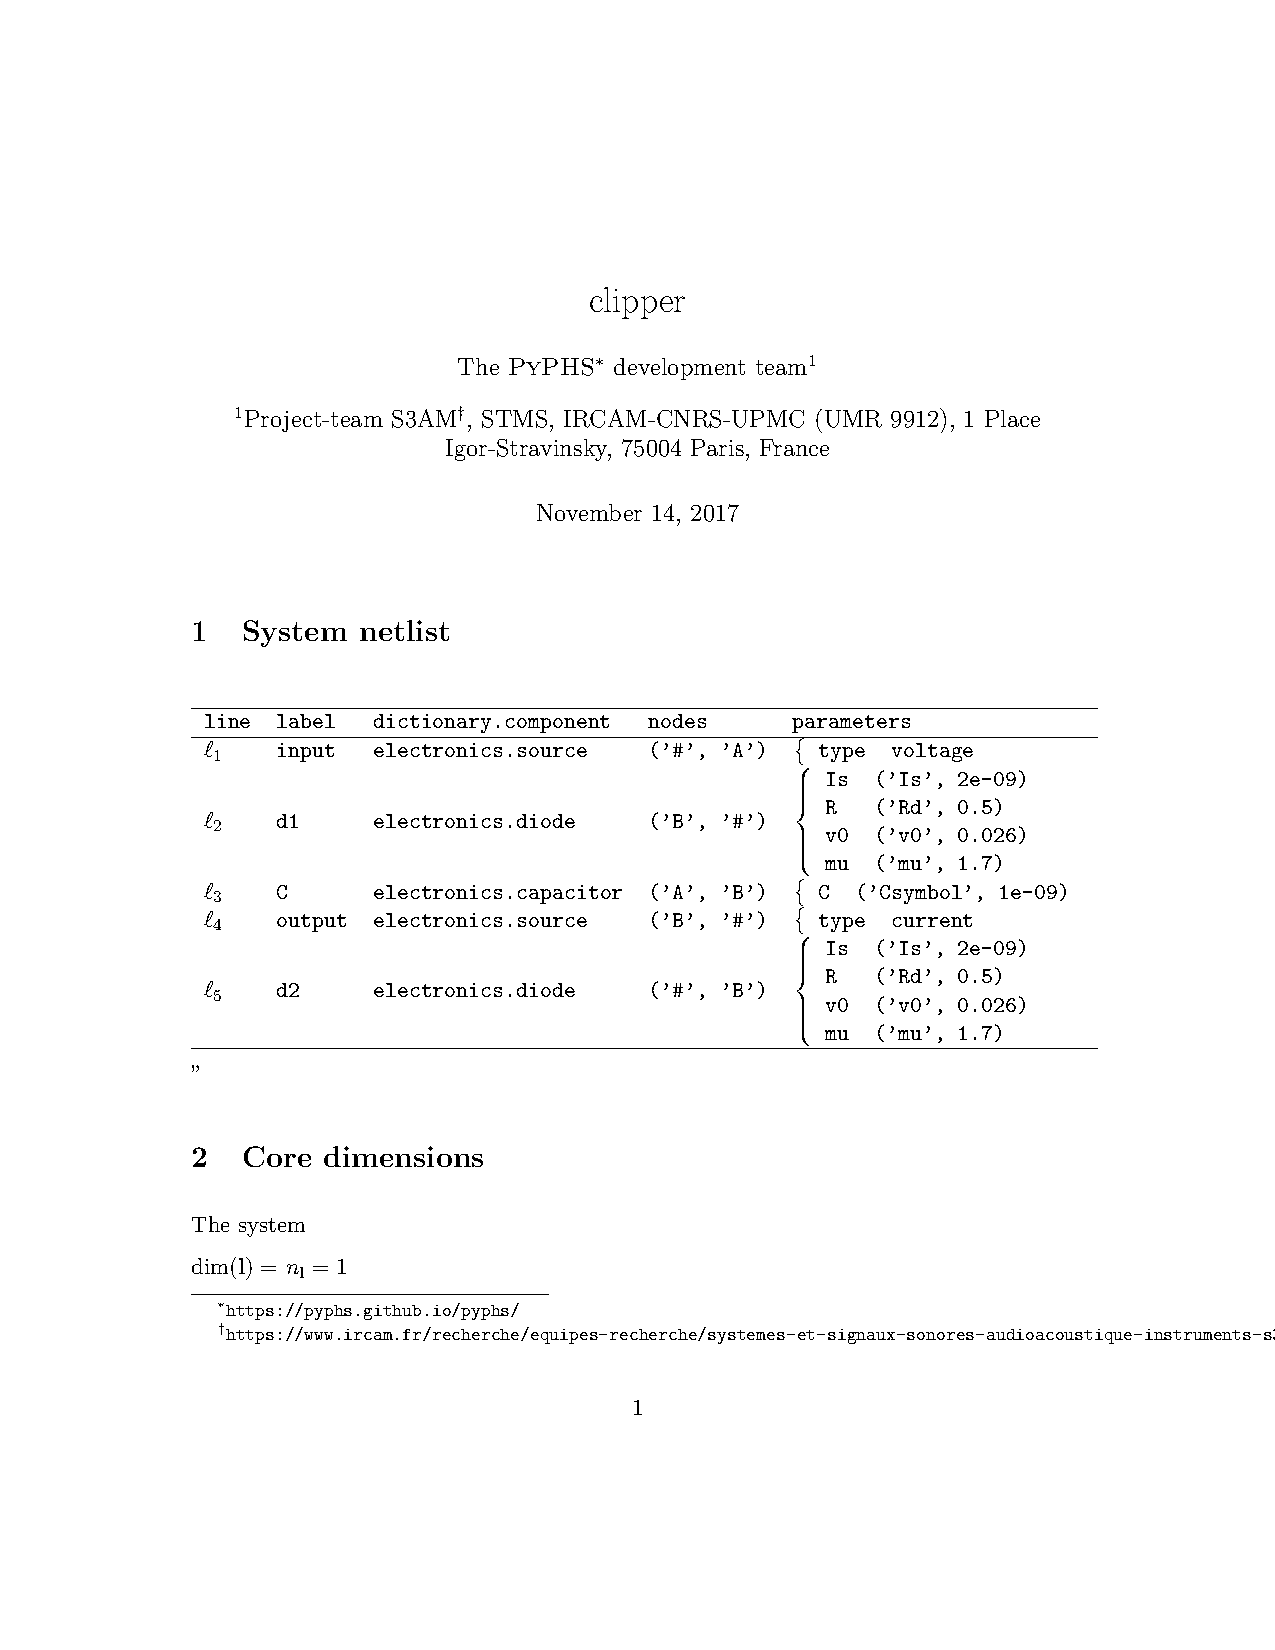
\includegraphics[width=\linewidth]{/Users/afalaize/Developement/repos/pyphs_gui/pyphs_gui/clipper.pdf}
%
\caption{\label{fig:graphclipper} Graph of system \texttt{clipper}. }
\end{center}
\end{figure}
%
%
%
"\section{Core dimensions}

The system

$\dim(\mathbf{l})=$ $ n_\mathbf{l} = 1$ \par $\dim(\mathbf{n_l})=$ $ n_\mathbf{n_l} = 2$ \par $\dim(\mathbf{x})=$ $ n_\mathbf{x} = 1$ \par $\dim(\mathbf{x_l})=$ $ n_\mathbf{x_l} = 1$ \par $\dim(\mathbf{x_nl})=$ $ n_\mathbf{x_nl} = 0$ \par $\dim(\mathbf{w})=$ $ n_\mathbf{w} = 2$ \par $\dim(\mathbf{w_l})=$ $ n_\mathbf{w_l} = 0$ \par $\dim(\mathbf{w_nl})=$ $ n_\mathbf{w_nl} = 2$ \par $\dim(\mathbf{y})=$ $ n_\mathbf{y} = 2$ \par $\dim(\mathbf{p})=$ $ n_\mathbf{p} = 0$ \par $\dim(\mathbf{o})=$ $ n_\mathbf{o} = 0$ \par $\dim(\mathbf{cy})=$ $ n_\mathbf{cy} = 0$ \par 
%
%
\section{Core quantities}
%
%
\subsection{Core constants}
%
\begin{center}
%
\begin{tabular}{ll}
%
\hline
parameter & value (SI)
\\ \hline
$I_{\mathrm{s}}$ & 2e-09
\\
$R_{\mathrm{d}}$ & 0.5
\\
$v_{\mathrm{0}}$ & 0.026
\\
$m_{\mathrm{u}}$ & 1.7
\\
$g_{\mathrm{min}}$ & 1e-12
\\
$C_{\mathrm{symbol}}$ & 1e-09
\\
\hline
\end{tabular}
%
\end{center}
%


\subsection{Core variables}

The system variables are:


\begin{itemize}


\item the \emph{state} $\mathbf x: t\mapsto \mathbf x(t)\in \mathbb R ^{1}$ associated with the system's energy storage:


$$ \mathbf{x} = \left(\begin{array}{c}x_{\mathrm{C}}\end{array}\right)$$


\item the \emph{state increment} $\mathbf{d_x}: t\mapsto \mathbf{d_x}(t)\in \mathbb R ^{1}$ that represents the numerical increment during a single simulation time-step:


$$ \mathbf{d_x} = \left(\begin{array}{c}d_{\mathrm{xC}}\end{array}\right)$$


\item the \emph{dissipation variable} $\mathbf w: t\mapsto \mathbf w(t)\in \mathbb R^{2}$ associated with the system's energy dissipation:


$$ \mathbf{w} = \left(\begin{array}{c}w_{\mathrm{d1}}\\w_{\mathrm{d2}}\end{array}\right)$$


\end{itemize}



\subsection{Core inputs}

The input (\textit{i.e.} controlled quantities) are:


\begin{itemize}


\item the \emph{input variable} $\mathbf u: t\mapsto \mathbf u(t)\in \mathbb R^{2}$ associated with the system's energy supply (sources):


$$ \mathbf{u} = \left(\begin{array}{c}u_{\mathrm{output}}\\u_{\mathrm{input}}\end{array}\right)$$


\item the \emph{parameters} $\mathbf p: t\mapsto \mathbf p(t)\in \mathbb R^{0}$ associated with variable system parameters:


$$ \mathbf p = \mathrm{Empty}$$


\end{itemize}



\subsection{Core outputs}

The output (\textit{i.e.} observed quantities) are:


\begin{itemize}


\item the \emph{output variable} ${\mathbf y: t\mapsto \mathbf y(t)\in \mathbb R^{2}}$ associated with the system's energy supply (sources):


$$ \mathbf y = \left(\begin{array}{c}y_{\mathrm{output}}\\y_{\mathrm{input}}\end{array}\right)$$


\item the \emph{observer} ${\mathbf o: t\mapsto \mathbf o(t)\in \mathbb R^{0}}$ associated with functions of the above quantities:


$$ \mathbf o = \mathrm{Empty}$$

\end{itemize}


\subsection{Core connectors}

The connected quantities are:


\begin{itemize}


\item the \emph{connected inputs} ${\mathbf u_c: t\mapsto \mathbf u_c(t)\in \mathbb R^{0}}$


$$ \mathbf u_c = \mathrm{Empty}$$


\item the \emph{connected outputs} ${\mathbf y_c: t\mapsto \mathbf y_c(t)\in \mathbb R^{0}}$


$$ \mathbf y_c = \mathrm{Empty}$$

\end{itemize}

%

%
%
\section{Core constitutive relations}

\subsection{Core storage function}

The system's storage function is:


$$ \mathrm H(\mathbf{x}) = \frac{0.5}{C_{\mathrm{symbol}}} \cdot x_{\mathrm{C}}^{2}$$


The gradient of the system's storage function is:


$$ \nabla\mathrm H(\mathbf{x}) = \left(\begin{array}{c}g_{\mathrm{xC}}\end{array}\right)$$

The elements of the storage function's gradient are given below:
$$ g_{\mathrm{xC}} = \frac{1.0}{C_{\mathrm{symbol}}} \cdot x_{\mathrm{C}}$$
    

The Hessian matrix of the storage function is:


$$ \triangle\mathrm H(\mathbf x) = \left(\begin{array}{c}\frac{1.0}{C_{\mathrm{symbol}}}\end{array}\right)$$

%
%

The Hessian matrix of the linear part of the storage function is:


$$ \mathbf{Q} = \left(\begin{array}{c}\frac{1.0}{C_{\mathrm{symbol}}}\end{array}\right)$$

%
%


\subsection{Core dissipation function}

The dissipative function is:


$$ \mathbf z(\mathbf{w}) = \left(\begin{array}{c}z_{\mathrm{d1}}\\z_{\mathrm{d2}}\end{array}\right)$$

%
%

The elements of the dissipation function are given below:
$$ z_{\mathrm{d1}} = I_{\mathrm{s}} \cdot \left(e^{\frac{w_{\mathrm{d1}}}{m_{\mathrm{u}} \cdot v_{\mathrm{0}}}} - 1\right)$$

%
$$ z_{\mathrm{d2}} = I_{\mathrm{s}} \cdot \left(e^{\frac{w_{\mathrm{d2}}}{m_{\mathrm{u}} \cdot v_{\mathrm{0}}}} - 1\right)$$

%

The jacobian matrix of the dissipation function is:

%

$$ \mathcal J_{\mathbf z}(\mathbf w) = \left(\begin{array}{cc}\frac{I_{\mathrm{s}} \cdot e^{\frac{w_{\mathrm{d1}}}{m_{\mathrm{u}} \cdot v_{\mathrm{0}}}}}{m_{\mathrm{u}} \cdot v_{\mathrm{0}}} & 0\\0 & \frac{I_{\mathrm{s}} \cdot e^{\frac{w_{\mathrm{d2}}}{m_{\mathrm{u}} \cdot v_{\mathrm{0}}}}}{m_{\mathrm{u}} \cdot v_{\mathrm{0}}}\end{array}\right)$$

%
%

The jacobian matrix of the linear part of the dissipation function is:


$$ \mathbf{Z_l} = \left(\begin{array}{cccc}g_{\mathrm{min}} & 0 & 0 & 0\\0 & g_{\mathrm{min}} & 0 & 0\\0 & 0 & R_{\mathrm{d}} & 0\\0 & 0 & 0 & R_{\mathrm{d}}\end{array}\right)$$

%
%

\section{Core structure}


$$
\left(
\begin{array}{c}
\frac{\mathrm d\, \mathbf x}{\mathrm d t} \\
\mathbf w \\
\mathbf y \\
\end{array}
\right)
=
\left(
\begin{array}{lll}
\mathbf{M_{xx}} & \mathbf{M_{xw}} & \mathbf{M_{xy}} \\
\mathbf{M_{wx}} & \mathbf{M_{ww}} & \mathbf{M_{wy}} \\
\mathbf{M_{yx}} & \mathbf{M_{yw}} &  \mathbf{M_{yy}} \\
\end{array}
\right)
\cdot
\left(
\begin{array}{c}
\nabla \mathrm H\\
\mathbf z \\
\mathbf u \\
\end{array}
\right)
$$

%

$$
\underbrace{\left(
\begin{array}{lll}
\mathbf{M_{xx}} & \mathbf{M_{xw}} & \mathbf{M_{xy}} \\
\mathbf{M_{wx}} & \mathbf{M_{ww}} & \mathbf{M_{wy}} \\
\mathbf{M_{yx}} & \mathbf{M_{yw}} &  \mathbf{M_{yy}} \\
\end{array}
\right)}_{\mathbf M}
=
\underbrace{\left(
\begin{array}{lll}
\mathbf{J_{xx}} & \mathbf{J_{xw}} & \mathbf{J_{xy}} \\
-^\intercal\mathbf{J_{xw}} & \mathbf{J_{ww}} & \mathbf{J_{wy}} \\
-^\intercal\mathbf{J_{xy}} & -^\intercal\mathbf{J_{wy}} &  \mathbf{J_{yy}} \\
\end{array}
\right)}_{\mathbf J}
-
\underbrace{\left(
\begin{array}{lll}
\mathbf{R_{xx}} & \mathbf{R_{xw}} & \mathbf{R_{xy}} \\
^\intercal\mathbf{R_{xw}} & \mathbf{R_{ww}} & \mathbf{R_{wy}} \\
^\intercal\mathbf{R_{xy}} & ^\intercal\mathbf{R_{wy}} &  \mathbf{R_{yy}} \\
\end{array}
\right)}_{\mathbf R}
$$

%
\subsection{Core M-structure}
%
$$ \mathbf{M} = \left(\begin{array}{ccccc}- \frac{2.0 \cdot g_{\mathrm{min}}}{R_{\mathrm{d}} \cdot g_{\mathrm{min}} + 1} & \frac{1.0}{R_{\mathrm{d}} \cdot g_{\mathrm{min}} + 1} & - \frac{1.0}{R_{\mathrm{d}} \cdot g_{\mathrm{min}} + 1} & 1.0 & - \frac{2.0 \cdot g_{\mathrm{min}}}{R_{\mathrm{d}} \cdot g_{\mathrm{min}} + 1}\\- \frac{1.0}{R_{\mathrm{d}} \cdot g_{\mathrm{min}} + 1} & - \frac{1.0 \cdot R_{\mathrm{d}}}{R_{\mathrm{d}} \cdot g_{\mathrm{min}} + 1} & 0 & 0 & - \frac{1.0}{R_{\mathrm{d}} \cdot g_{\mathrm{min}} + 1}\\\frac{1.0}{R_{\mathrm{d}} \cdot g_{\mathrm{min}} + 1} & 0 & - \frac{1.0 \cdot R_{\mathrm{d}}}{R_{\mathrm{d}} \cdot g_{\mathrm{min}} + 1} & 0 & \frac{1.0}{R_{\mathrm{d}} \cdot g_{\mathrm{min}} + 1}\\-1.0 & 0 & 0 & 0 & -1.0\\- \frac{2.0 \cdot g_{\mathrm{min}}}{R_{\mathrm{d}} \cdot g_{\mathrm{min}} + 1} & \frac{1.0}{R_{\mathrm{d}} \cdot g_{\mathrm{min}} + 1} & - \frac{1.0}{R_{\mathrm{d}} \cdot g_{\mathrm{min}} + 1} & 1.0 & - \frac{2.0 \cdot g_{\mathrm{min}}}{R_{\mathrm{d}} \cdot g_{\mathrm{min}} + 1}\end{array}\right)$$
%
$$ \mathbf{M_{xx}} = \left(\begin{array}{c}- \frac{2.0 \cdot g_{\mathrm{min}}}{R_{\mathrm{d}} \cdot g_{\mathrm{min}} + 1}\end{array}\right)$$
%
$$ \mathbf{M_{xw}} = \left(\begin{array}{cc}\frac{1.0}{R_{\mathrm{d}} \cdot g_{\mathrm{min}} + 1} & - \frac{1.0}{R_{\mathrm{d}} \cdot g_{\mathrm{min}} + 1}\end{array}\right)$$
%
$$ \mathbf{M_{xy}} = \left(\begin{array}{cc}1.0 & - \frac{2.0 \cdot g_{\mathrm{min}}}{R_{\mathrm{d}} \cdot g_{\mathrm{min}} + 1}\end{array}\right)$$
%
$$ \mathbf{M_{xcy}} = \mathrm{Empty}$$
%
$$ \mathbf{M_{wx}} = \left(\begin{array}{c}- \frac{1.0}{R_{\mathrm{d}} \cdot g_{\mathrm{min}} + 1}\\\frac{1.0}{R_{\mathrm{d}} \cdot g_{\mathrm{min}} + 1}\end{array}\right)$$
%
$$ \mathbf{M_{ww}} = \left(\begin{array}{cc}- \frac{1.0 \cdot R_{\mathrm{d}}}{R_{\mathrm{d}} \cdot g_{\mathrm{min}} + 1} & 0\\0 & - \frac{1.0 \cdot R_{\mathrm{d}}}{R_{\mathrm{d}} \cdot g_{\mathrm{min}} + 1}\end{array}\right)$$
%
$$ \mathbf{M_{wy}} = \left(\begin{array}{cc}0 & - \frac{1.0}{R_{\mathrm{d}} \cdot g_{\mathrm{min}} + 1}\\0 & \frac{1.0}{R_{\mathrm{d}} \cdot g_{\mathrm{min}} + 1}\end{array}\right)$$
%
$$ \mathbf{M_{wcy}} = \mathrm{Empty}$$
%
$$ \mathbf{M_{yx}} = \left(\begin{array}{c}-1.0\\- \frac{2.0 \cdot g_{\mathrm{min}}}{R_{\mathrm{d}} \cdot g_{\mathrm{min}} + 1}\end{array}\right)$$
%
$$ \mathbf{M_{yw}} = \left(\begin{array}{cc}0 & 0\\\frac{1.0}{R_{\mathrm{d}} \cdot g_{\mathrm{min}} + 1} & - \frac{1.0}{R_{\mathrm{d}} \cdot g_{\mathrm{min}} + 1}\end{array}\right)$$
%
$$ \mathbf{M_{yy}} = \left(\begin{array}{cc}0 & -1.0\\1.0 & - \frac{2.0 \cdot g_{\mathrm{min}}}{R_{\mathrm{d}} \cdot g_{\mathrm{min}} + 1}\end{array}\right)$$
%
$$ \mathbf{M_{ycy}} = \mathrm{Empty}$$
%
$$ \mathbf{M_{cyx}} = \mathrm{Empty}$$
%
$$ \mathbf{M_{cyw}} = \mathrm{Empty}$$
%
$$ \mathbf{M_{cyy}} = \mathrm{Empty}$$
%
$$ \mathbf{M_{cycy}} = \mathrm{Empty}$$
%
\subsection{Core J-structure}
%
$$ \mathbf{J} = \left(\begin{array}{ccccc}0 & \frac{1.0}{R_{\mathrm{d}} \cdot g_{\mathrm{min}} + 1} & - \frac{1.0}{R_{\mathrm{d}} \cdot g_{\mathrm{min}} + 1} & 1.0 & 0\\- \frac{1.0}{R_{\mathrm{d}} \cdot g_{\mathrm{min}} + 1} & 0 & 0 & 0 & - \frac{1.0}{R_{\mathrm{d}} \cdot g_{\mathrm{min}} + 1}\\\frac{1.0}{R_{\mathrm{d}} \cdot g_{\mathrm{min}} + 1} & 0 & 0 & 0 & \frac{1.0}{R_{\mathrm{d}} \cdot g_{\mathrm{min}} + 1}\\-1.0 & 0 & 0 & 0 & -1.0\\0 & \frac{1.0}{R_{\mathrm{d}} \cdot g_{\mathrm{min}} + 1} & - \frac{1.0}{R_{\mathrm{d}} \cdot g_{\mathrm{min}} + 1} & 1.0 & 0\end{array}\right)$$
%
$$ \mathbf{J_{xx}} = \mathrm{Zeros}$$
%
$$ \mathbf{J_{xw}} = \left(\begin{array}{cc}\frac{1.0}{R_{\mathrm{d}} \cdot g_{\mathrm{min}} + 1} & - \frac{1.0}{R_{\mathrm{d}} \cdot g_{\mathrm{min}} + 1}\end{array}\right)$$
%
$$ \mathbf{J_{xy}} = \left(\begin{array}{cc}1.0 & 0\end{array}\right)$$
%
$$ \mathbf{J_{xcy}} = \mathrm{Empty}$$
%
$$ \mathbf{J_{wx}} = \left(\begin{array}{c}- \frac{1.0}{R_{\mathrm{d}} \cdot g_{\mathrm{min}} + 1}\\\frac{1.0}{R_{\mathrm{d}} \cdot g_{\mathrm{min}} + 1}\end{array}\right)$$
%
$$ \mathbf{J_{ww}} = \mathrm{Zeros}$$
%
$$ \mathbf{J_{wy}} = \left(\begin{array}{cc}0 & - \frac{1.0}{R_{\mathrm{d}} \cdot g_{\mathrm{min}} + 1}\\0 & \frac{1.0}{R_{\mathrm{d}} \cdot g_{\mathrm{min}} + 1}\end{array}\right)$$
%
$$ \mathbf{J_{wcy}} = \mathrm{Empty}$$
%
$$ \mathbf{J_{yx}} = \left(\begin{array}{c}-1.0\\0\end{array}\right)$$
%
$$ \mathbf{J_{yw}} = \left(\begin{array}{cc}0 & 0\\\frac{1.0}{R_{\mathrm{d}} \cdot g_{\mathrm{min}} + 1} & - \frac{1.0}{R_{\mathrm{d}} \cdot g_{\mathrm{min}} + 1}\end{array}\right)$$
%
$$ \mathbf{J_{yy}} = \left(\begin{array}{cc}0 & -1.0\\1.0 & 0\end{array}\right)$$
%
$$ \mathbf{J_{ycy}} = \mathrm{Empty}$$
%
$$ \mathbf{J_{cyx}} = \mathrm{Empty}$$
%
$$ \mathbf{J_{cyw}} = \mathrm{Empty}$$
%
$$ \mathbf{J_{cyy}} = \mathrm{Empty}$$
%
$$ \mathbf{J_{cycy}} = \mathrm{Empty}$$
%
\subsection{Core R-structure}
%
$$ \mathbf{R} = \left(\begin{array}{ccccc}\frac{2.0 \cdot g_{\mathrm{min}}}{R_{\mathrm{d}} \cdot g_{\mathrm{min}} + 1} & 0 & 0 & 0 & \frac{2.0 \cdot g_{\mathrm{min}}}{R_{\mathrm{d}} \cdot g_{\mathrm{min}} + 1}\\0 & \frac{1.0 \cdot R_{\mathrm{d}}}{R_{\mathrm{d}} \cdot g_{\mathrm{min}} + 1} & 0 & 0 & 0\\0 & 0 & \frac{1.0 \cdot R_{\mathrm{d}}}{R_{\mathrm{d}} \cdot g_{\mathrm{min}} + 1} & 0 & 0\\0 & 0 & 0 & 0 & 0\\\frac{2.0 \cdot g_{\mathrm{min}}}{R_{\mathrm{d}} \cdot g_{\mathrm{min}} + 1} & 0 & 0 & 0 & \frac{2.0 \cdot g_{\mathrm{min}}}{R_{\mathrm{d}} \cdot g_{\mathrm{min}} + 1}\end{array}\right)$$
%
$$ \mathbf{R_{xx}} = \left(\begin{array}{c}\frac{2.0 \cdot g_{\mathrm{min}}}{R_{\mathrm{d}} \cdot g_{\mathrm{min}} + 1}\end{array}\right)$$
%
$$ \mathbf{R_{xw}} = \mathrm{Zeros}$$
%
$$ \mathbf{R_{xy}} = \left(\begin{array}{cc}0 & \frac{2.0 \cdot g_{\mathrm{min}}}{R_{\mathrm{d}} \cdot g_{\mathrm{min}} + 1}\end{array}\right)$$
%
$$ \mathbf{R_{xcy}} = \mathrm{Empty}$$
%
$$ \mathbf{R_{wx}} = \mathrm{Zeros}$$
%
$$ \mathbf{R_{ww}} = \left(\begin{array}{cc}\frac{1.0 \cdot R_{\mathrm{d}}}{R_{\mathrm{d}} \cdot g_{\mathrm{min}} + 1} & 0\\0 & \frac{1.0 \cdot R_{\mathrm{d}}}{R_{\mathrm{d}} \cdot g_{\mathrm{min}} + 1}\end{array}\right)$$
%
$$ \mathbf{R_{wy}} = \mathrm{Zeros}$$
%
$$ \mathbf{R_{wcy}} = \mathrm{Empty}$$
%
$$ \mathbf{R_{yx}} = \left(\begin{array}{c}0\\\frac{2.0 \cdot g_{\mathrm{min}}}{R_{\mathrm{d}} \cdot g_{\mathrm{min}} + 1}\end{array}\right)$$
%
$$ \mathbf{R_{yw}} = \mathrm{Zeros}$$
%
$$ \mathbf{R_{yy}} = \left(\begin{array}{cc}0 & 0\\0 & \frac{2.0 \cdot g_{\mathrm{min}}}{R_{\mathrm{d}} \cdot g_{\mathrm{min}} + 1}\end{array}\right)$$
%
$$ \mathbf{R_{ycy}} = \mathrm{Empty}$$
%
$$ \mathbf{R_{cyx}} = \mathrm{Empty}$$
%
$$ \mathbf{R_{cyw}} = \mathrm{Empty}$$
%
$$ \mathbf{R_{cyy}} = \mathrm{Empty}$$
%
$$ \mathbf{R_{cycy}} = \mathrm{Empty}$$
%

%
\end{document}